\section{Algorithm}

\begin{frame}{Getting started}
    \framesubtitle{What do we need?}
	\stress{Quantify \enquote{similar}} {\color{purple}(\emph{metric})}:\\
	$\lra$ Similarity test\\
    $\phantom{\lra}$ {\small e.g. $\chi^2$ test, Kolmogorov test, \dots}
	
	
	
	\bigskip
	\stress{Build up groups} {\color{purple}(\emph{clusters})} of similar distributions:\\
	$\lra$ Clustering algorithm\\
    $\phantom{\lra}$ {\small e.g. Hierarchical clustering, \dots}
	
    \bigskip
    \stress{Select representatives} {\color{purple}(\emph{benchmark points})} from each cluster
    
	\bigskip
	\stress{How many} clusters do we want?\\
	$\lra$ Add experimental error expectation\\
	$\lra$ Keep as many clusters as we can distinguish
\end{frame}

\begin{frame}[t]{Example: Hierarchical Clustering}
	\vspace{0.5cm}
   \centering
	\only<+>{
		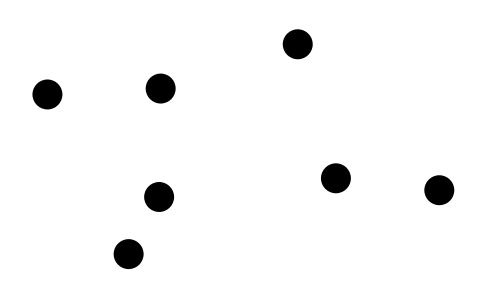
\includegraphics[width=10cm]{figures/hierarchy/step0.pdf}\\[2ex]
		Step 0: 7 points in the parameter space
	}
	\only<+>{
		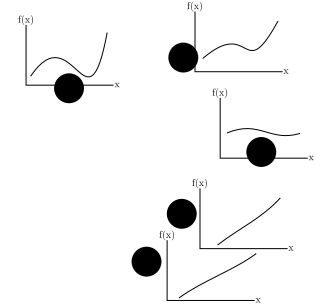
\includegraphics[width=10cm]{figures/hierarchy/step0_curves.pdf}\\[2ex]
		Step 0: 7 points in the parameter space = 7 distributions
	}
	\only<+>{
		\includegraphics[width=10cm]{figures/hierarchy/step1_curves.pdf}\\[2ex]
		Step 1: Every point is its own cluster
	}
	\only<+>{
		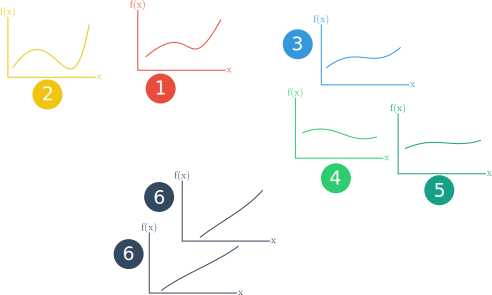
\includegraphics[width=10cm]{figures/hierarchy/step2_curves.pdf}\\[2ex]
		Step 1: Distributions from cluster 6 and 7 were the most similar $\Lra$ Merged!
	}
	\only<+>{
		\includegraphics[width=10cm]{figures/hierarchy/step3_curves.pdf}\\[2ex]
		Step 1: Cluster 4 and 5 were the next most similar clusters $\Lra$ Merged!
	}
	\only<+>{
		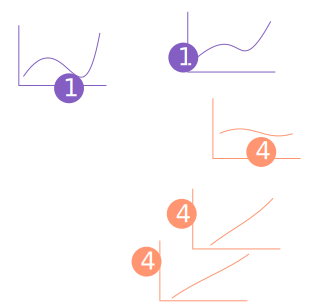
\includegraphics[width=10cm]{figures/hierarchy/step4_curves.pdf}\\[2ex]
		Step 1: 4 clusters remaining
	}
	\only<+>{
		\includegraphics[width=10cm]{figures/hierarchy/step5_curves.pdf}\\[2ex]
		Step 1: 3 clusters remaining
	}
	\only<+>{
		\includegraphics[width=10cm]{figures/hierarchy/step6_curves.pdf}\\[2ex]
		Step 1: 2 clusters remaining
	}
	\only<+>{
		\includegraphics[width=10cm]{figures/hierarchy/step7_curves.pdf}\\[2ex]
		Step 1: 1 cluster remaining
	}
	
%	}
\end{frame}